%% FELthesis: LaTeX class for bachelor, master, and phd thesis in CTU FEL
%% template.tex: template file
%% (c) 2012-2014 Vít Zýka, vit.zyka@seznam.cz
%%
%% 2012-12-17 v0.1 first version derived from cmpthesis.tex

\documentclass[msc,draft, czech]{felthesis} % or [...,czech] for thesis in Czech

%% --- your additional packages:
\usepackage[utf8]{inputenc}

%% --- usefull draft packages
%%\usepackage[notref]{showkeys} % show labels for referencies
%%\usepackage{showlabels}       % similar
%%\usepackage{showidx}          % show index entries on every page

%% ======================================================== thesis info
\startThesisInfo
  \Title{Metody automatizace testů síťových prvků}
  \Author{Bc. David Felgr}
  \AuthorEmail{felgrdav@fel.cvut.cz} % optional
  \Date{May 2015}
  \Department{Katedra Měření}
  \Advisor{Ing. Pavel kopecký, doc. Ing. Jiří Novák, Ph.D.}
  \KeywordsCz{První klíčové slovo; druhé; třetí; \dots}
  \KeywordsEn{First keyword; second; third; \dots}
  %\AssignmentPage{assignment.pdf} % insert official assignment if given
\stopThesisInfo

%% ============================== your definitions (abbreviations etc.)
%%\def\Ax{\mathbf{A}_{x}}

%% =========================================================== settings
\addbibresource{\jobname.bib} % bibliography file
\graphicspath{{logo/}{images/}} % subdirectories where TeX finds pictures
\DeclareGraphicsExtensions{.pdf,.png,.jpg}
%% ========================================================== text body
\begin{document}

\MakeTitle

\startFrontMatter
  \startAcknowledgement
Chtěl bych poděkovat svému vedoucímu diplomové práce doc. Ing. Jiřímu Novákovi, Ph.D. za prvotní nasměrování při řešení problému. Dále bych chtěl poděkovat kolegům ve~vývojovém oddělení za cenné rady při realizaci testovacího systému i při jazykové korekci práce.
\stopAcknowledgement

\endinput
%%
%% End of file `acknowledgement.tex'.

  \startDeclaration
\ifCzech
  Prohlašuji, že jsem předloženou práci vypracoval samostatně,
  a~že jsem uvedl veškeré použité informační zdroje v~souladu
  s~Metodickým pokynem o~dodržování etických principů při přípravě
  vysokoškolských závěrečných prací.
\fi
\ifEnglish
  I declare that I worked out the presented thesis independently
  and I quoted all used sources of information in accord with
  Methodical instructions about ethical principles for writing
  academic thesis.
\fi
\stopDeclaration

\endinput
%%
%% End of file `declaration.tex'.

  \startAbstractCz
Tento dokument ukazuje a testuje použití oficiálně doporučené \LaTeX{}ové šablony
\FelThesis{} pro sazbu bakalářské, diplomové a disertační práce na
Elektrotechnické fakultě ČVUT. Šablona definuje všechny povinné
strukturní elementy zmíněných závěrečných prací a formátuje jejich
obsah tak, aby splňovala na škole daná formální pravidla.
\stopAbstractCz

\startAbstractEn
This document shows and tests an usage of the \LaTeX{} officially
recommended design style \FelThesis{} for bachelor (Bsc.), master
(Ing.), or doctoral (Ph.D.) thesis at the Faculty of Electrical
Engineering of the Czech Technical University in Prague.
The template defines all thesis mandatory structural elements and
typesets their content to fulfil the university formal rules.
\stopAbstractEn

\endinput

  \TableOfContents
  \font\mflogo=logo10
\def\METAFONT{{\mflogo META}\-{\mflogo FONT}}
\def\METAPOST{{\mflogo META}\-{\mflogo POST}}
\hyphenation{Post-Script}

\startAbbreviations{%
  As an example of an abbreviation description serve some terms from
  TeX{} world. This introductory paragraph is optional and can stay empty.}
\label{abbrv}%
\abbrv[\TeX{}]  Typesetting program and macro language by Donald Knuth.
\abbrv[\METAFONT{}] Program and macro language for font creation by
  Donald Knuth.
\abbrv[\METAPOST{}] Vector drawing program based on \METAFONT{} with
  Encapsulated PostScript output by John Hobby.
\abbrv[plain \TeX{}]  Original \TeX{} format (macro extension) by
Donald Knuth. User customization is done by programing in \TeX{} macro language.
\abbrv[\LaTeX{}]  Most known and used \TeX{} format originally by
  Leslie Lamport. There is a huge number of packages that extends
  standard functionality or bypass programing in \TeX{}. User
  customization is primarily done by loading predefined class or
  package and rewriting their definitions.
\abbrv[Con\TeX{}t]  Complex typesetting and vector drawing system based
  on \TeX{}, \METAPOST{} and Lua script language by Hans Hagen. Customization is
  done by key-value parametrization with conjunction to \TeX{},
  \METAPOST{} and Lua programing.
\stopAbbreviations

\setlength{\AbbrvIndent}{2em}

\startAbbreviations*[Symbols]{%
  The abbreviation environment starts a new page. If we want to avoid
  page break like in this second short list use starred version {\tt\Backslash
  startAbbreviations*}. Indentation might be adjusted by the command
  {\tt\Backslash setlength\{\Backslash AbbrvIndent\}\{5em\}} to be
  appropriate to the symbols width.}
\abbrv[$\pi$] Final version number of \TeX{}.
\abbrv[e] Final version number of \METAFONT{}.
\abbrv[$2\varepsilon$] Version of today's \LaTeX{} valid since 1994. It
  was intended as a temporary intermediate version between original
  Leslie Lamports's last version \LaTeX{} 2.09 and \LaTeX{}3 that is
  developed as its successor.
\stopAbbreviations

\endinput
%%
%% End of file `abbreviation.tex'.

\stopFrontMatter

\startBodyMatter
  \chapter{Úvod}
Tématem této diplomové práce jsou metody automatizace testů síťových prvků. Nejdříve bychom měl popsat definici testování a různé způsoby jak je možné testování provádět. Definice testování je podle IEEE Software Engineering Body of Knowledge (SWEBOK 2004) následující:

"Softwarové testování se skládá z dynamického ověřování chování programu proti očekávanému chování programu na konečné množině testovacích případů vhodně vybraných z obvykle nekonečné množiny případů."

Na způsoby testování lze pohlížet několika pohledy. Prvním pohledem na testování je rozdělení na šest jednotlivých úrovní testování. Mezi tyto úrovně testování patří testování programátorem, testování jednotlivých jednotek kódu, funkční testování, integrační testování, systémové testování a akceptační testy. Všechny úrovně budou detailně popsány v kapitole používané metody testování. Dalším pohledem na kategorizaci testování je způsob provádění testů. Prvním způsobem je manuální testování, kdy tester manuálně provádí testy podle předem daných testovacích procedur. Dokonalejším způsobem testování je takzvané automatizované testování, kdy testy jsou prováděny automaticky dle předem napsaných testovacích procedur. Testovací procedury jsou psány testery či vývojáři. Všechny testovací procedury musí být přepisovány při změně funkcionality výrobku, nebo při přidání nového výrobku. Tímto přístupem je ušetřeno spoustu času, který byl plýtván opakovaným manuálním testováním identických věcí. Posledním známým a v dnešní době moderním způsobem testování je testování založené na modelech. U tohoto způsobu testování je vytvořen model testované oblasti, či zařízení a automaticky se generují testovací procedury. Způsob testování založeného na modelech ušetří další čas trávený úpravami a tvorbou dalších testovacích procedur při změně funkcionality softwaru či přidání nového produktu, jelikož je upravován pouze model zařízení. Testovací systém, který bude výstupem této diplomové práce, by měl testovat zařízení na úrovni systémového testování. Systémové testy by měl testovací systém pro konkrétní zařízení vybírat a  provádět automatizovaně pomocí testování založeného na modelech.

\section{Praktické využití}
Praktická implementace testovacího systému bude provedena pro testování výrobků společnosti Conel, ze které přišel požadavek na toto zadání. Zadání diplomové práce jsem si vybral, jelikož ve společností pracuji na různých pozicích již 4 roky. Způsoby testování výrobku se během fungování firmy měnily následujícím způsobem. Zpočátku, kdy počet modelů routerů byl velmi malý a routery vyvíjel pouze jeden programátor bylo prováděno pouze testování programátorem a následovali až akceptační testy u zákazníka. Při rostoucím počtu modelů, funkcionalit a počtu vývojářů byl tento systém již dále neudržitelný a mezi testy programátorem a akceptačními testy musely být vloženy systémové testy prováděny testerem podle testovacích procedur. Dnes, kdy počet modelů routerů přesahuje 30 základních modelů a nové funkcionality  přibývají čím dál tím rychleji, je tento systém taktéž dále neudržitelný. Již nyní by kompletní testování všech funkcionalit na všech typech routerů trvalo přibližně měsíc práce v jednom člověku.

\begin{figure}[h]
	\centering
	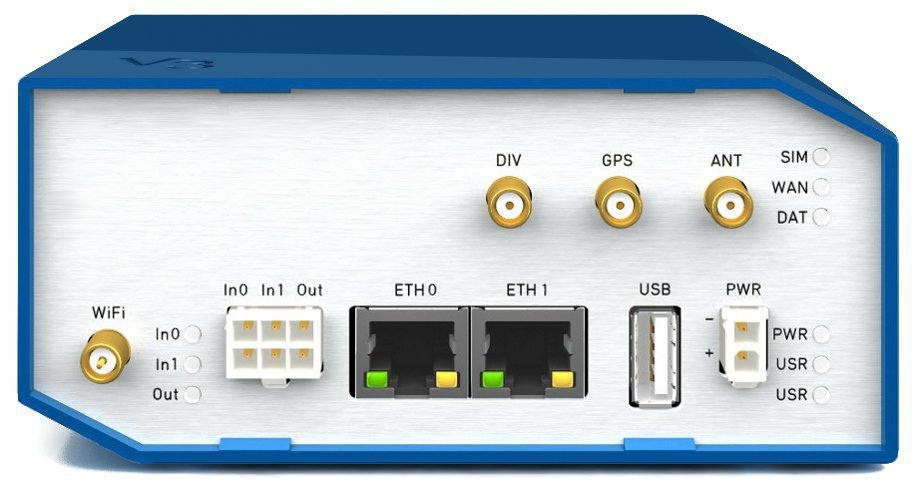
\includegraphics[width=.6\LW]{router}
	\caption{Příklad routeru}
	\label{fig:router}
\end{figure}

Na základě těchto skutečností byl vznešen požadavek na testovací systém, pomocí kterého bude možné automaticky testovat aktuálně vyvíjený firmware na všech vyráběných modelech routerů a jejich volitelných portech. Zvolena byla kombinace integračního testování a testování založené na modelech. Testování bude pokrývat pouze integrační a systémové testování, jelikož z větší části je firmware testovaných výrobků tvořen opensource programy. Psaní unit testů pro každý open source program je časově a složitostně nepřínosné. Systémové testování by mělo probíhat alespoň jednou denně, aby bylo možno případné chyby odchytnout již během vývoje firmwaru a tím usnadnilo a zrychlilo vývoj samotný. Dalším velikým přínosem je zkvalitnění samotného testování, jelikož testovací technici mohou vymýšlet nové testovací procedury a situace, namísto opakovaného manuálního testování stejných procedur.

\section{Aktuálnost}
Testování každého výrobku před uvedením na trh, či testováním nového firmwaru před jeho vydáním je velmi důležitá součást vývoje a neměla by se opomíjet. Hlavním důvodem průběžného testování kompletní funkcionality zařízení je dobré jméno u zákazníka, který nemá zájem o výrobek plný chyb. Dalším důvodem průběžného testování je méně práce pří pozdějším opravování způsobených chyb. Při zvyšování počtu výrobků a funkcionalit je nutné zvyšovat počet testovacích pracovníků, nebo změnit přístup k způsobu testování. Jelikož první řešení se zdá být na první pohled neefektivní, tak se v této práci vydám druhou cestou. Při zvyšování efektivity testů použiju automatizované testování. Dále pokud to bude možné a alespoň trochu efektivní využiji dnes velmi moderní metodu testování založeného na modelech. Každému zařízení by měl být vytvořen model, pomocí kterého budou na určených zařízeních spouštěny vybrané testy s danými parametry. V dnešní době byrokracie tento systém také pomůže ke shromažďování všech testovacích procedur a reportů ze všech provedených testů na jednom místě.

\section{Výstup práce}
Hlavním cílem práce je hotové řešení automatizovaného systémového řešení testování všech modelů bezdrátových routerů společnosti Conel. Výstupem  řešení bude testovací laboratoř obsahující všechny výrobky, pomocné síťové prvky a testovací server. Dalším výstupem bude aplikace na obstarávající režii a spouštění testů, interface pro zobrazování reportů ze všech testů s možností administrace testovacího systému. Poslední cíl je vytvoření testovacích procedur pro testování jednotlivých funkcí bezdrátových routerů společnosti Conel.

\section{Struktura práce}
Celou diplomovou práci lze rozdělit do třech hlavních částí. V první teoretické částí budou rozebírány všechny různé metody a přístupy k testování samotnému, aby bylo možné dále stavět na teoretickém základu. Dále v teoretické části budou prozkoumány všechny možné dostupné produkty určené k samotnému testování, či produkty sloužící k jednotlivým úkonům potřebným pro testování daných produktů. Zde bude kladena snaha využít co nejvíce kvalitních hotových řešení sloužících k účelům testování výrobků společnosti Conel. Ideální cesta by byla nalézt produkt sloužící k našemu účelu, ale jelikož je požadavek velmi specifický, s velkou pravděpodobností bude potřeba z velké části testovací systém vyvinout. Druhá část práce se bude zabývat praktickým návrhem všech částí zabývající se testováním každého routeru. V první fázi bude navrhnuta testovací laboratoř z hlediska potřebného hardwaru. Dále bude popsán návrh a implementace programu zajišťující samotné testování a úkony s testováním související. Následuje kapitola věnující se uživatelskému interfacu pro reportování výsledků a administraci samotného testování. Samostatná kapitola popisuje api pro snadné dopisování nových testovacích procedur. Základní api bude dodáno s testovacím programem a dále bude popsána možnost dopisování nových specifických programů. Stěžejní části je kapitola popisující testovací procedury jednotlivých funkcionalit. Poslední částí je praktická implementace testovací laboratoře a testování celého systému. Výstupy z tohoto testování budou použity v poslední kapitole zabývající se možností budoucího vylepšení a rozšíření testovacího systému.

\endinput

  \chapter{Používané metody testování}
V této kapitole se pokusím popsat co nejvíce známých pohledů a způsobů na testování, aby bylo dále možné vybrat, aplikovat a navrhovat testovací systém s ohledem na dnešní metody a trendy v testování. Nejdříve popíšu úrovně testování, kterými by měl každý výrobek před uvedením na trh projít. Dále popíši způsoby  testování, kterými může testování proběhnout. V poslední kapitole jsou popsány další nezařazené možné pohledy a přístupy k testování.

\section{Úrovně testování}
Testování výrobků před uvedením na trh prochází několika stupni testování. Některé stupně jsou při vývoji používány bez toho, aby si to vývojáři uvědomili a jiné důležité stupně testování jsou zase často opomíjeny. Mnou rozebíraný model má celkem 5 stupňů testování. Jednotlivé stupně dále popíši a rozeberu jejich přínos a možnosti použití v mém testovacím systému.

\begin{figure}[h]
  \centering
  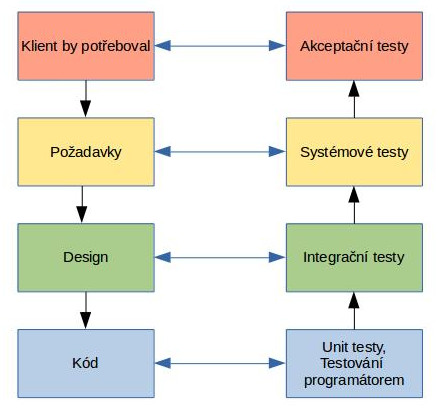
\includegraphics[width=.6\LW]{test_phase}
  \caption{Schéma testovacího modelu}
  \label{fig:test_phase}
\end{figure}

\subsection{Testování programátorem (Developer testing)}
První a úplně nezbytnou fázi testování by měli provádět programátoři. Programátor by si měl zkontrolovat jestli je možné firmware přeložit a dále jestli jeho nová či opravená funkcionalita funguje správně. V další fázi testování by měl zkontrolovat kód jiný programátor, který kód nepsal. Tuto fázi většinou provádí správce projektu při zařazování nové či upravené funkce do hlavní větve repozitáře projektu. Všechny chyby odchycené v této fázi testování ušetří spoustu času stráveném v dalších fázích testování.

Testování programátorem může vypadat jako samozřejmá věc, která by nemusela být ani uváděna. Bohužel opak je pravdou a i tato situace může nastat. V případě že je tato fáze vynechána je pravděpodobné že spousta chyb je odhaleno až ve fázi systémového testování, kdy zjišťování, reportování a oprava chyb stojí značnou režii.

\subsection{Testování jednotek (Unit testing)}
Úroveň testování jednotek obsahuje testování jednotlivých částí nebo modulů softwaru. Za jednotku neboli část lze považovat objekt s jednou jedinou funkcionalitou, a to například třídu, objekt, program či softwarový modul. Tato úroveň testování testuje správnost zdrojového kódu a ne funkci programu jako celku. Velmi známým příkladem jsou JUnit testy v javě, kde ke každé třídě a metodě je vytvářena testovací třída či metoda.

Unit testy je výhodné použít při tvorbě nového projektu, jelikož s unit testy je potřeba počítat již při návrhu zdrojového kódu a při návrhu kódu zároveň testy vytvářet. Dopisování testů do již existujícího projektu by stálo neúměrnou námahu a mnoho úprav kódu pro přizpůsobování samotného programu pro unit testování.

Zdrojový kód pro výrobky testované navrhovaným testovacím systémem je vyvíjen již 10 let a zároveň na těchto zdrojových kódech jsou stavěny i nové výrobky. Navíc přes devadesát procent firmwaru používá opensource řešení. Díky těmto dvěma skutečnostem je v nynější situaci nereálně přidat unit testování do navrhovaného testovacího schématu.

\subsection{Integrační testování (Integration testing)}
Po předchozích dvou úrovních testování, jenž jsou prováděny programátory, přichází fáze, kdy se hotový výrobek dostává do ruky testerům. Testeři většinou provádí dvě úrovně testování, integrační testování a systémové testování. Někdy jsou tyto dvě fáze spojovány do jedné a nazývají se systémově integrační testování. Obě úrovně budou dále detailněji popsány.

\begin{figure}[h]
  \centering
  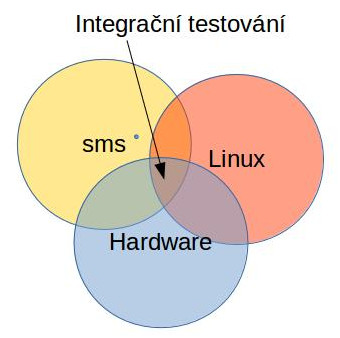
\includegraphics[width=.4\LW]{test_integration}
  \caption{Grafické znázornění integračního testování}
  \label{fig:test_integration}
\end{figure}

Pomocí integračního testování testujeme integraci jednotlivých komponent mezi ostatní komponenty, dále také integraci jednotlivých komponent do operačního systému, či na konkrétní hardware. Jako příklad mohu uvést testování integrace programu odesílání sms zpráv na operačním systému Linux, běžícím na hardwaru konkrétního routeru. Příklad znázorňuje, že není testováno pouze odesílání sms zpráv, ale komponenta v závislosti na operačním systému a hardwaru. Jednotlivé komponenty mohou být například subsystémy, databázové implementace, infrastruktura, rozhraní a systémové konfigurace. Integrační testování lze z testování vypustit, jelikož chyby nalezené v této fázi by byly odhaleny ve fázi systémového testování, nýbrž za cenu vyšší časové náročnosti.

Integrační testy navrhují testeři na základě čtyř základních skutečností a to softwárový a systémový design výrobku, architekturu firmwaru, pracovního postupu s danou komponentou a možnými případy použití. Na základě těchto čtyř skutečností tester navrhne testovací případy a postupy. Podle těchto postupů jsou jednotlivé komponenty dále testovány manuálně testery či automaticky automatem.

Testovací automat bude v prvním kroku testovat integračními testy všechny základní komponenty routeru, jako například posílání SMS zpráv, či SMPT klient vůči operačnímu systému Linux či uCLinux běžícím na každém z 50 různých výrobků podporujících testovanou funkcionalitu. Zde je nejlépe vidět přínos testovacího automatu. Ve skutečnosti by tester měl provést test integrace všech funkcionalit na všech padesáti odlišných výrobcích, což je časově značně náročné. Zatímco automat tento test může provést každý den na všech výrobcích paralelně během chvilky. Tímto testováním je ověřena integrace daného programu na všech výrobcích a neunikne žádná chyba způsobená chybou v firmwaru, či chybou některé ze součástí routeru, čímž může být například odlišná implementace odesílání sms v bezdrátovém modulu.

\subsection{SIT - Systémové testování (System testing)}
Systémové testování je poslední fází testování probíhající ve společnosti vyvíjecí daný produkt. Ve fázi systémového testování se testuje výrobek jako celek z pohledu zákazníka. Jsou navrhnuty jednotlivé testovací případy, které mohou nastat v praxi, a dle těchto případů jsou výrobky testovány. Příklad takového testovacího scénáře může být testovaný router do kterého je přes Ethernet připojena IP kamera a přes sériové rozhraní teplotní senzor. Data z těchto zařízení jsou přes OpenVPN tunel sestavený přes mobilní spojení posílána na vzdálený server.

\begin{figure}[h]
  \centering
  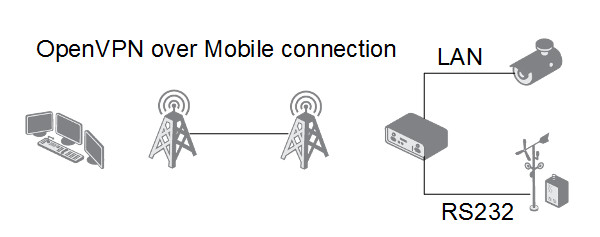
\includegraphics[width=.8\LW]{system_test_example}
  \caption{Příklad systémového testování}
  \label{fig:system_test_example}
\end{figure}

Systémové testy mohou obsahovat funkční i nefunkční testy, které jsou dále popsané v sekci věnované těmto typům testování. Dále je možné testovat kvalitu či rychlost přenosu dat, které mohou být prováděny na výrobcích ve standartním, ale i ve stiženém prostředí, například v klimatické komoře nebo v okolí EMC vyzařovaní. Na systémové testování je také možné pohlížet jako na testování bílé či černé skříňky. Oba způsoby jsou také dále popsány v kapitole věnující se dalším typům testování.

V navrhovaném případě testování bude systémové testování prováděno ve stejném kroku a pomocí stejných nástrojů jako integrační testování, čili tento model se blíží dříve zmíněné možnosti spojení systémových a integračních testů. V navrhovaném případě testování lze někdy určit hranici mezi systémovými a integračními testy a někdy je toto rozdělení obtížné určit. Většina systémových testů obdobně jako integrační testy bude možné provádět automaticky pomocí testovacího automatu. Jiné systémové testy, jako například testy v klimatické komoře, budou muset být dále z kapacitních důvodů prováděny manuálně, jelikož všech padesát výrobků se do klimatické komory nevejde. Naopak tyto testy nezávisí na změně firmwaru, čili ve většině případech stačí pouze jedno provedení klimatických testů při vyvinutí nového hardwaru výrobku a ne při každé změně firmwaru.

\subsection{UAT - Akceptační testování (Acceptance testing)}
Poslední úrovní testování je akceptační testování. Akceptační testování již není prováděno testery ve firmě, kde je výrobek vyvíjen. Testování je prováděno u cílového zákazníka na konkrétní aplikaci výrobku. Případné chyby či nesrovnalosti od požadované funkcionality jsou reportovány zpět a bývá očekávána rychlá reakce na opravu těchto chyb. Snaha testovacího systému samozřejmě bude odhalit všechny případné chyby před touto úrovní, tedy před dodáním výrobku zákazníkovy. Jelikož se tato fáze provádí až u koncového zákazníka, práce se touto fází dále nebude zabývat.

\section{Testovací procesy}
Fáze systémového a integračního testování lze provádět pomocí třech různých přístupů k testování. Všechny tři přístupy se od sebe liší hlavně v délce a složitosti návrhu testování a v délce samotného provádění testů. V neposlední řadě se liší jejich pokrytí testovacích případů a tím i kvalita testování. Podle složitosti návrhu testů by bylo možné popisované přístupy testování seřadit sestupně na testování založené na modelech, automatizované testování a poslední manuální testování. Rychlostí a efektivitou provádění testů jsou tyto způsoby seřazeny přesně opačně. Cílem této práce je automatizovat a tím zkrátit provádění testů a zároveň rozšířit možností testování. Z cíle práce tedy vyplývá, že se budu snažit pokusit o přechod z nynějšího manuálního testování na automatizované testování a v nejlepším případě na testování založené na modelech.

\subsection{Manuální testování}
Prvním přístupem provádění testů je manuální testování. Manuální testování je možné rozdělit do dvou nezávislých kroků. Prvním krokem každého manuálního testování je vytvoření testovacího plánu. Testovací plán obsahuje informace o tom, co by mělo být na výrobku testováno, jak by měl být výrobek testován a nakonec jak často by měl být výrobek testován. Dle tohoto plánů navrhuje testovací technik testovací scénáře a jejich jednotlivé testovací procedury. Navrhování testovacích procedur se provádí pokaždé při změně nebo přidání nějaké funkcionality výrobku. Návrh provádí testovací technik s požadovanými znalostmi o testovaném výrobku.

\begin{figure}[h]
  \centering
  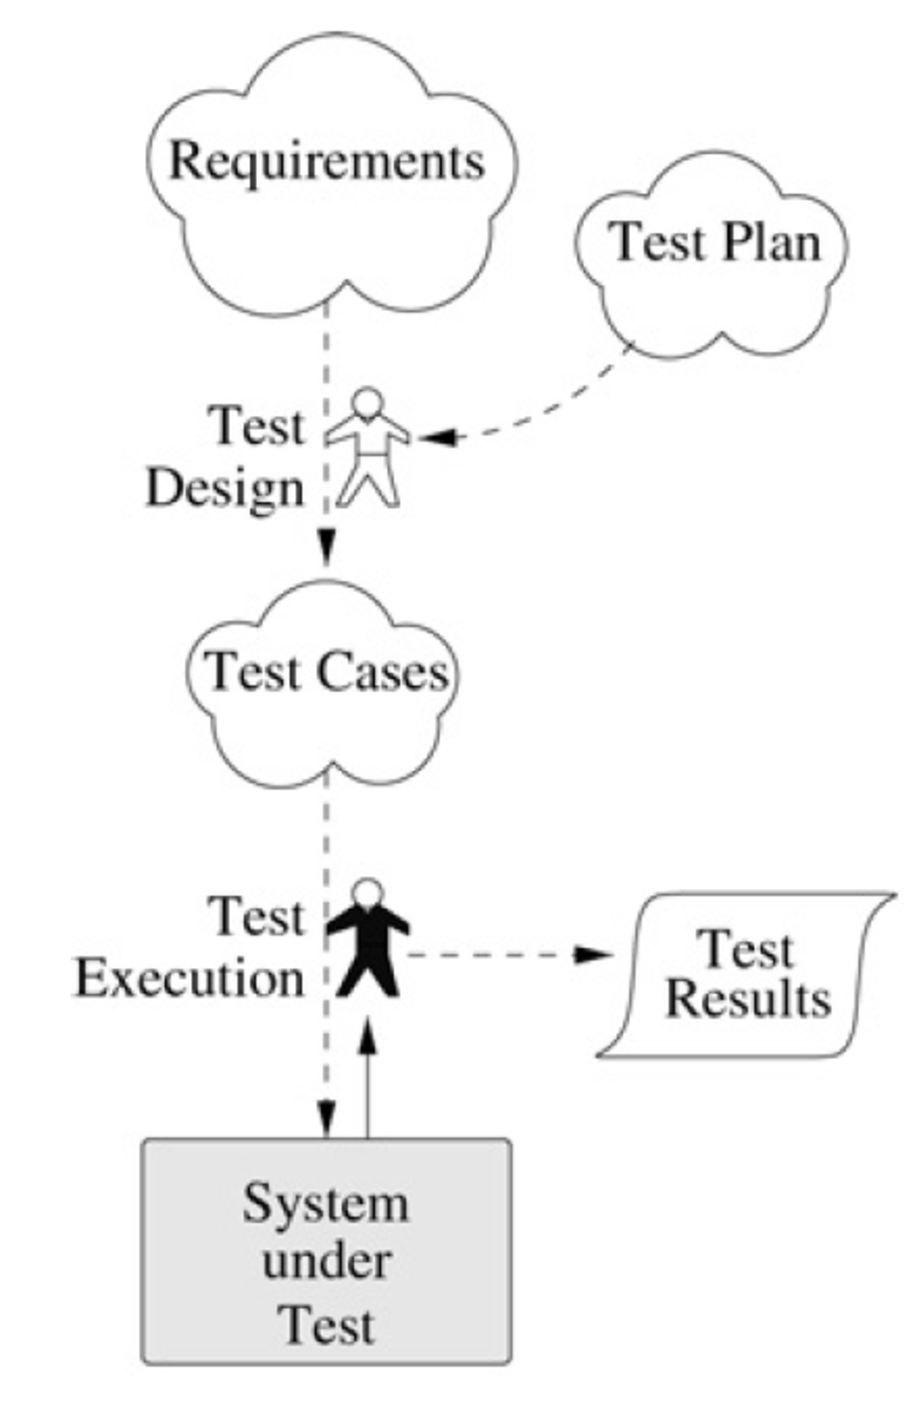
\includegraphics[width=.4\LW]{test_manual}
  \caption{Schéma manuálního testování}
  \label{fig:test_manual}
\end{figure}

Druhou fází manuálního testování je samotné provádění testů. Testy se provádějí manuálně přímo na testovaném objektu podle předepsaných testovacích procedur. Provádění testů je opakováno při každé změně ve firmwaru výrobku a dle jeho komplexnosti bývá i velice časově náročný. Z toho důvodu bývají některé testy vypouštěny, ale na úkor kvality testování celého výrobku. Samotné testování je práce manuální dle předepsaných pokynů a také velmi často se opakující, z toho plyne, že tuto práci může vykonávat tester bez znalostí návrhu testování samotných výrobků a jejich technologií. Dále se tento proces přímo nabízí k nějakému zlepšení jakoukoliv automatizací.

Ve společnosti, kde bude testovací systém nasazován, se nyní všechny testy provádějí manuálně dle předepsaných testovacích procedur. Jak už bylo v úvodu zmíněno, při rychle rostoucím počtu výrobků a jejich funkcionalit je nadále tento systém testování neudržitelný. Provádění integračních a systémových testů se budu snažit přesunout do jednoho ze sofistikovanějších způsobů testování. Dále pro specifické testy jako například EMC testy a klimatické testy v teplotní komoře nebude z kapacitních důvodů možné plně automatizovat a bude možné navrhnout moduly pro zjednodušené manuální testování.

Mohou nastávat i případy manuálního testování, kdy nejsou vytvořeny testovací plány a testovací procedury, kde možné později doložit adekvátní výsledky testování. Další nevýhodou tohoto přístupu k testování je vynechání velkého množství testovacích případů, jelikož se jedná spíše o náhodné testování, proto tento postup není určitě doporučován.

\subsection{Automatizované testování}
Druhým a sofistikovanějším způsobem provádění testů je automatizované testování, někdy také nazývané testování založené na skriptech. Automatizované testování lze rozdělit do třech základních fází. První fáze vytvoření testovacího plánu je shodná s manuálním testováním.

\begin{figure}[h]
  \centering
  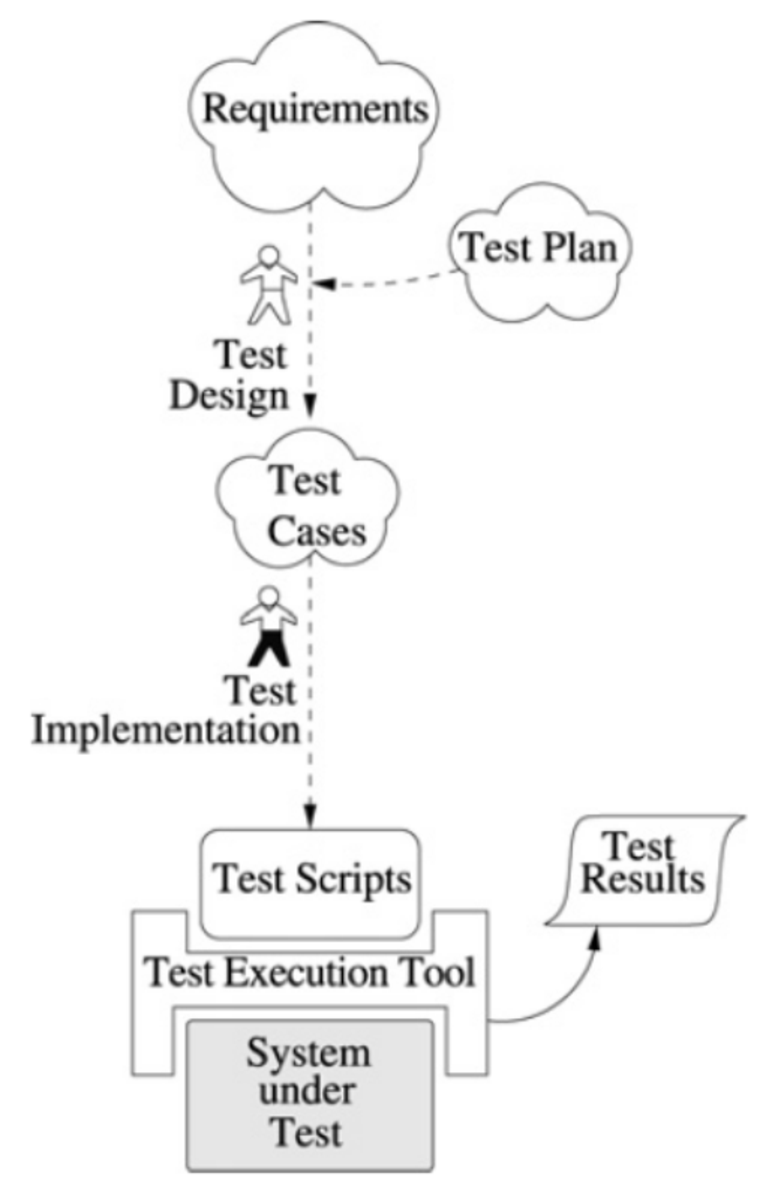
\includegraphics[width=.4\LW]{test_automat}
  \caption{Schéma automatického testování}
  \label{fig:test_automat}
\end{figure}

Druhou fází automatického testování je implementace testovacích procedur do spustitelných skriptů. Skriptovací testy mohou být napsány v nějakém standardním programovacím či skriptovacím jazyku nebo v jazyku přímo určenému k psaní testovacích skriptů. V našem systému bude k psaní testovacích skriptů použit skriptovací jazyk Bash a jednoduché programy napsané v programovací jazyk C. V automatizovaném přístupu testování nám přibyla další role programátora potřebného k implementaci testovacích procedur do spustitelných skriptů. Testovací skript je spustitelný skript nebo program, který provede jednu testovací proceduru. Testovací skript obvykle obsahuje inicializaci testovacího zařízení, uvedení testovacího zařízení do požadovaného kontextu, vytvoření vstupních testovacích hodnot, předání vstupních hodnot do testovaného zařízení, nahrání odpovědi od testovaného zařízení, nakonec porovnání odpovědi a očekávaného výstupu a vyhodnocení výsledku.

Třetí fází automatického testování je automatické spouštění testů. Testy jsou spouštěny automaticky pomocí nástroje pro spouštění testů. Nástroj provádí spouštění testů automaticky bez interakce s obsluhou. Nástroj navíc obsahuje možnost paralelizace testů nezávislých na nějakém zdroji. Zde je vidět veliká časová a tedy i finanční úspora oproti manuálnímu testování. Jestliže chceme provést nový test zařízení, spustíme pouze testovací nástroj a není potřeba manuálně testovat všechny funkcionality.

Naopak tento přístup přináší větší režii při změně funkcionality či přidání nového zařízení. Pokud je změněna testovací procedura či přímo funkcionalita výrobku, musí být předělány a přidány testovací skripty. Tato údržba může být v případech intenzivního vývoje stejně časově nákladná jako tvorba nových testovacích procedur pro danou funkcionalitu.

\subsection{Testování založené na modelech}
Nejsofistikovanějším řešením testování je testování založené na modelech, známé taky jako MBT (Model Base Testing). Zjednodušeně lze model tohoto systému popsat následovně. Tester vytvoří model testovaného zařízení, z tohoto modelu se automaticky vygenerují testovací skripty, které jsou spouštěny nad testovaným výrobkem. U tohoto testování odpadá spoustu času při návrhu a úpravách testovacích skriptů. Naproti tomu je velmi časově náročné navrhnutí samotného testovacího systému a modelu testovaného výrobku. Samozřejmě, že všechno není tak jednoduché, jak se na první pohled zdá a tak dále jsou detailně popsány všechny fáze tohoto způsobu testování. Jednotlivé fáze MBT jsou vývoj modelu testovaného zařízení, generování abstraktních testů z modelu, převedení abstraktních testů na spustitelné testy, spuštění testů na testovaném zařízení a analýza výsledků testů.

\begin{figure}[h]
  \centering
  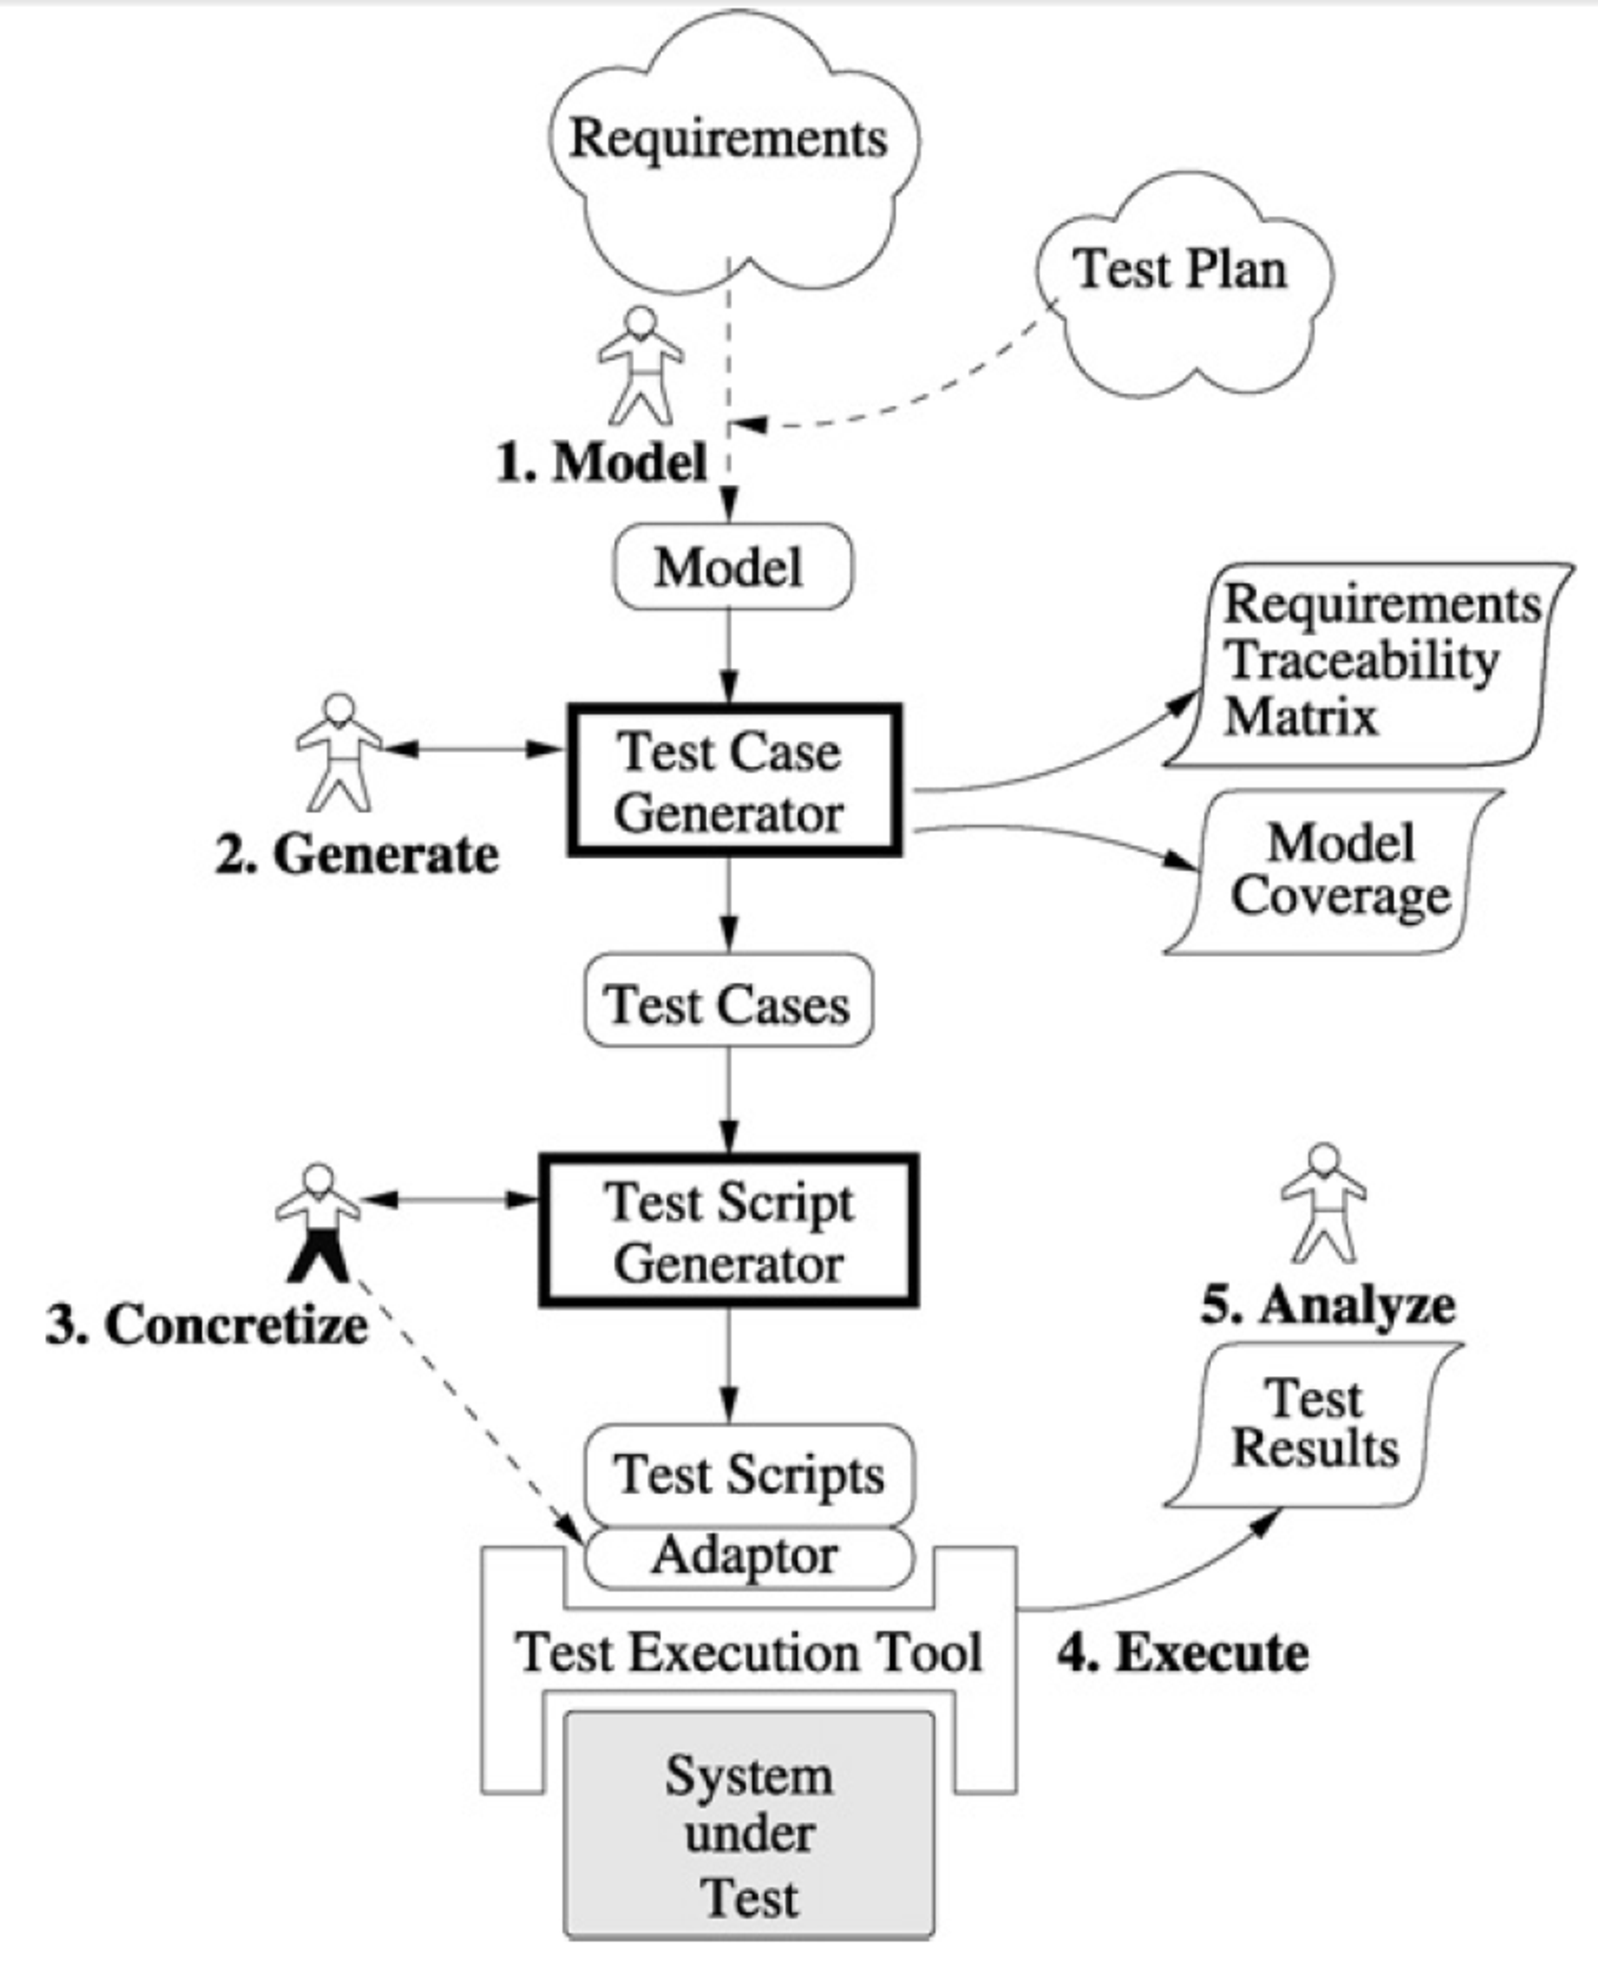
\includegraphics[width=.5\LW]{test_model}
  \caption{Schéma testování založeného na modelech}
  \label{fig:test_model}
\end{figure}

Prvním krokem testování založeném na modelech je tedy vytvoření abstraktního modelu testovaného zařízení. Model by měl být jednodušší nežli samotné zařízení a měl by se zaměřit na jeho klíčové vlastnosti.

Druhým krokem testování založeném na modelech je generování abstraktních testů z hotového modelu. Jelikož by ve většině případů bylo vygenerováno nekonečné množství testovacích případů, tak je potřeba určit nějaké testovací kritéria, aby bylo možné vygenerovat konečné množství testů. Tyto testy jsou sekvencí operací nad modelem. Používají zjednodušený pohled na testované zařízení a nejsou přímo spustitelné.

Třetí částí testování založeném na modelech je transformace abstraktních testů na spustitelné konkrétní testy. Transformace může být prováděna dvěma způsoby. Prvním způsobem je transformační nástroj, který používá šablony a mapuje každý abstraktní testovací případ do spustitelného skriptu. Nebo je možné napsat adaptér kódu, který implementuje každou abstraktní operaci jako operaci nad testovaném zařízení a doplní jí detaily, které nejsou navrženy v abstraktním modelu.

Ve čtvrtém kroku jsou spouštěny konkrétní testy na testovaném systému. Tato fáze je shodná s třetí fází automatizovaného testování. Tedy může používat stejný systém a ve zjednodušené variantě lze říci, že jde pouze o jiné generování testovacích skriptů. Dále jde tento krok rozdělit na online a offline testování. Při online testování se generují testy při každém spuštění testu. Při offline testování jsou testy předem generovány a pokud nenastane změna v testovacím modelu, jsou používány stejné již předem generované testy.

V posledním pátém kroku se analyzují výsledky spuštěných testů a jejich korektní chování. V případě neúspěšného kroku se analyzuje příčina a místo vzniku chyby. Nejčastější místa vzniku chyby jsou chybný model, chybný adaptér kódu a v neposlední řadě může chyba vzniknout chybnou funkcí testovaného výrobku.

Z popisu tohoto způsobu testování je vidět, že v případě správné implementace tohoto systému na testovaný produkt by mohlo výrazně usnadnit práci při testování. Samotná implementace je velmi složitá a ne všechny testované objekty lze efektivně popsat tímto systémem. Nasazení systému testování založeného na modelech ztroskotalo po několika letech i ve velkých společnostech jako například IBM. V testovacím systému pro výrobky společnosti Conel bude snaha použít systém testování založeného na modelech alespoň  na  nevyšší abstraktní úrovni.

\section{Typy testování}
Poslední podkapitola typy testů probírá pojmy z testování, které nebyly obsaženy v žádném z předchozích modelů a v testování se občas používají či naopak je některý z předchozí modelů používá a nebyly detailně popsány.

\subsection{Testy splněním a selháním}
Testy splněním používají vstupní data pouze množinu dat, které testovaný systém musí správně vyhodnotit, taktéž se chováme k systému korektním způsobem, při tom kontrolujeme jestli odpověď od testovaného systému se shoduje s očekávanou odpovědí. Naopak při testech selháním zacházíme s testovaným systémem nekorektně a na vstup mu přivádíme data, které systém neumí vyhodnotit a kontrolujeme jestli systém nespadl či systém nevrací odpověď shodující se s očekávaným výstupem.

\subsection{Progresní a regresní testy}
Progresními testy nazýváme testy kontrolující nové funkce testovaného výrobku. K sestavení progresních testů je nutná znalost nových funkcí daného výrobku. Regresními testy se nazývá opětovné testování již testovaných vlastností výrobků. Regresní testy jsou často prováděny při dokončení části vývoje pro ujištění, zda-li nové úpravy neovlivňují jiné části firmwaru. Taktéž jsou prováděny před vydáním nového firmwaru.

\subsection{Smoke testy}
Smoke testy je označení testů obsahující pouze jednoduché testování spustitelnosti produktu a jeho základních funkcionalit. Většinou se toto testování provádí před systémovými testy. Největší význam těchto testů přichází ve výrobě nových produktů pro ověření funkčnosti vyrobeného výrobků.

\subsection{Funkční a nefunkční testy}
Pomocí funkčních testů jsou testovány všechny funkce implementované v testovaném výrobku a jejich správné fungování. Tyto testy jsou popisovány v předchozích kapitolách. Další metodou jsou často opomíjené nefunkční testy testující funkce výrobku přímo nesouvisející s jeho funkcionalitou. Jedná se například o testování výkonu celého výrobku nebo jeho částí. Kontroluje se zde jestli výrobek dosahuje požadovaného výkonu a zároveň jestli je při zvýšené zátěži stále dobře funkční.

\subsection{Testování bílé a černé skříňky}
Testování bílé skříňky je prováděno, pokud při navrhování testů má tester přístup a využívá zdrojových kódu testovaného výrobku. Naopak při testování černé skříňky tester zdrojové kódy k dispozici nemá a k návrhu testů využívá pouze dokumentace k danému výrobku.

\subsection{Statické a dynamické testy}
Statické testy nepotřebují ke svému provádění spuštěný program. Naopak dynamické testy ke svému fungování potřebují spuštěný funkční program.

\endinput

  \chapter{Dostupné testovací nástroje}
V kapitole dostupné testovací nástroje popíšu zkoumanou část dostupných opensource i komerčních nástrojů pro jednotlivé fáze testování. U všech testovacích nástrojů bude posuzován přínos v případě nasazení v testovacím systému pro výrobky společnosti Conel.

\section{Jenkins CI}
Jenkins CI je nástroj pro kontinuální integraci. Kontinuální integrace spočívá v častém kompilování zdrojového kódu a následném spouštění testů nad tímto softwarem.
Jenkins CI je nástroj napsaný v programovacím jazyce Java. Tento nástroj má podporu  kompilace různých projektů díky veliké možnosti nastavení a velké podpoře v podobě rozšiřujících pluginů, jejichž počet neustále roste.

\begin{figure}[h]
  \centering
  
\includegraphics[width=.3\LW]{jenkins_logo}
  \caption{Logo produktu http://www.jenkins-ci.org}
  \label{fig:testlink_logo}
\end{figure}

Jenkinsen je dobrý a přehledný buildovací systém s podporou mnoha programovacích jazyků. Velikou výhodou tohoto systému je opensource řešení projektu, naopak nevýhodou jsou veliké systémové požadavky nástroje. Tento systém sice podporuje testování, ale podporuje pouze testování na úrovní testování jednotek, které v navrhovaném systému nebude vůbec využito. Jenkins CI naopak nepodporuje funkční a systémové testování na konkrétním hardwaru, které je v testovacím systému vyžadováno.

\begin{figure}[h]
  \centering
  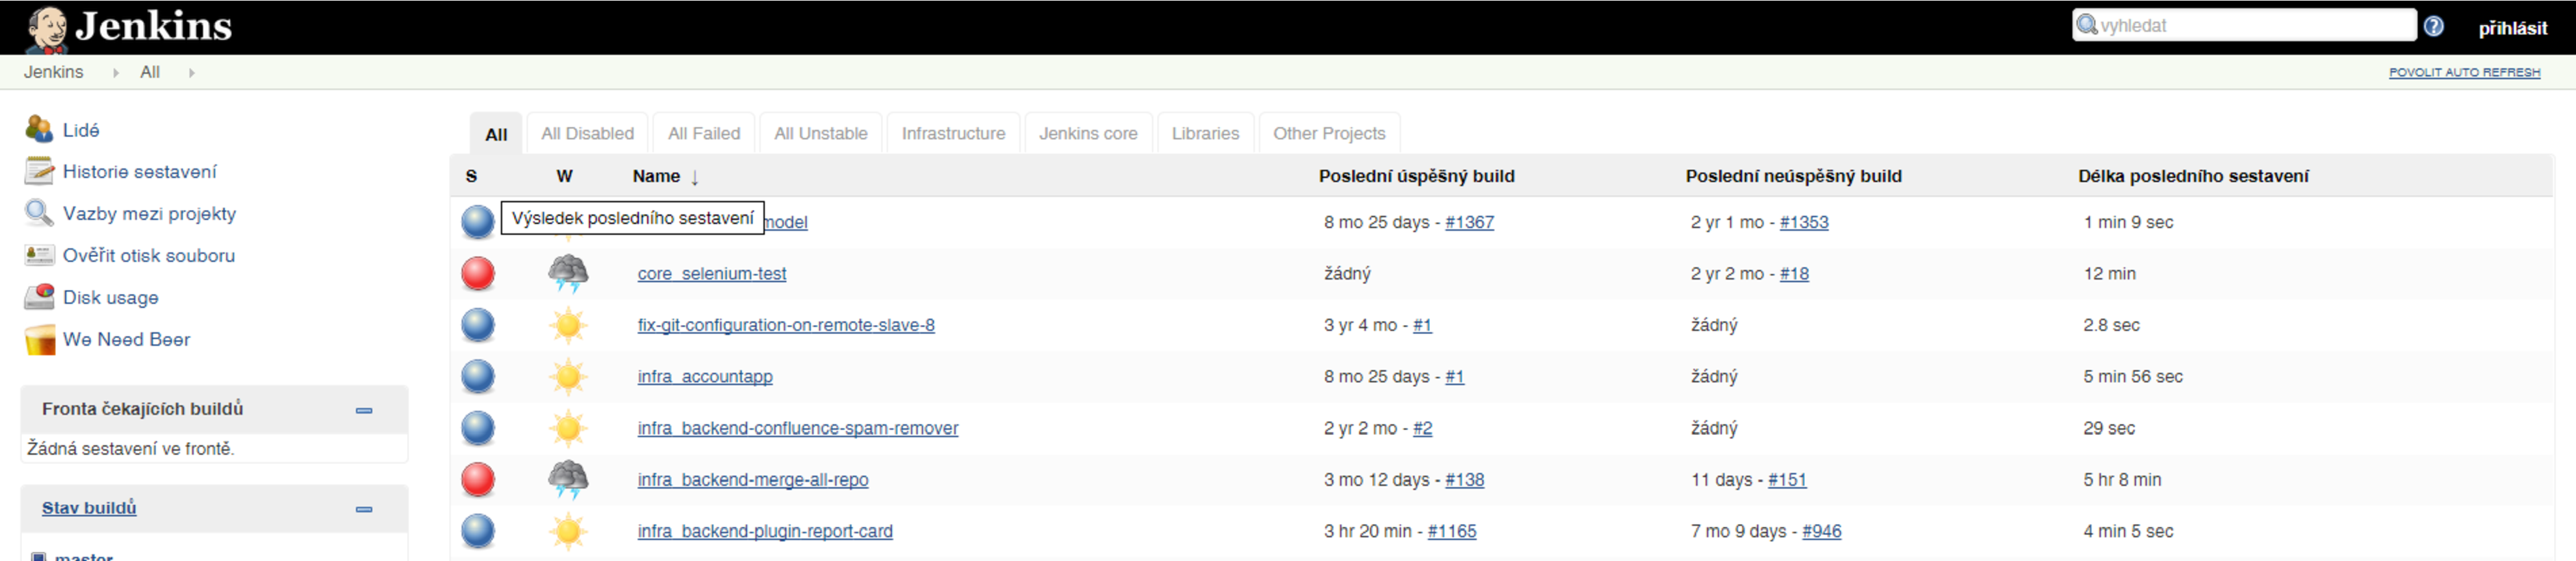
\includegraphics[width=\LW]{jenkins_example}
  \caption{Příklad otevřené aplikace Jenkinsen}
  \label{fig:testlink_example}
\end{figure}

Použití nástroje Jenkins CI pro kontinuální integraci v testovacím zařízení by bylo možné pouze ve fázi buildování všech firmwarů. Skripty zajišťující správnou funkci s buildovacím program ltib je potřeba napsat stejné jak při použití systému Jenkins, tak při vlastním spouštění překladu. LTIB je image systém používající se pro překlad většiny testovaných výrobků. Taktéž samotné spouštění těchto skriptů bude v testovacím systému již implementováno v části obsluhující spouštění testovacích skriptů. Na základě těchto skutečností jsem upřednostnil použití vlastního spouštění kompilačních skriptů, hlavně z důvodu jednotného systému pro vizualizaci všech informací o průběhu všech fází překladu a testování.

\section{Testlink}
Testlink je nástroj pro správu a organizaci testů. Nástroj je vytvořený jako webová aplikace napsaná v jazyce PHP využívající databázi MySQL nebo PostgeSQL. Aplikace je zdarma i pro komerční účely, jelikož je šiřená pod licencí GPL.

\begin{figure}[h]
  \centering
  
\includegraphics[width=.3\LW]{testlink_logo}
  \caption{Logo produktu http://www.testlink.org}
  \label{fig:testlink_logo}
\end{figure}

Nástroj testlink umí spravovat a organizovat testy a testovací případy. Testlink obsahuje pět základních pilířů, o které se dále opírá a tvoří jeho strukturu. Prvním a základním prvkem je testovací případ neboli test case. Testovací případlze přirovnat k skriptu či testovací proceduře popisované ve způsobech testování. Dalším prvkem je sada testů označovaná test suite. Sada testů organizuje testy do funkčních skupin. Třetím prvkem nástroje testlink je testovací plán. Testovací plán je sestaven ze sad testů a dále z dalších informací o daném testování. Dalším prvkem je testovací projekt, který je základním prvkem systému. Testovací projekt v známé terminologii odpovídá testovanému subjektu. Posledním prvkem tohoto systému je uživatel. Jednotlivý uživatelé mají různá práva úprav v systému, aby byla zavedena bezpečnost systému. Tento systém umí také podle vložených výsledků testů vytvářet reporty o testování v různých formátech.

\begin{figure}[h]
  \centering
  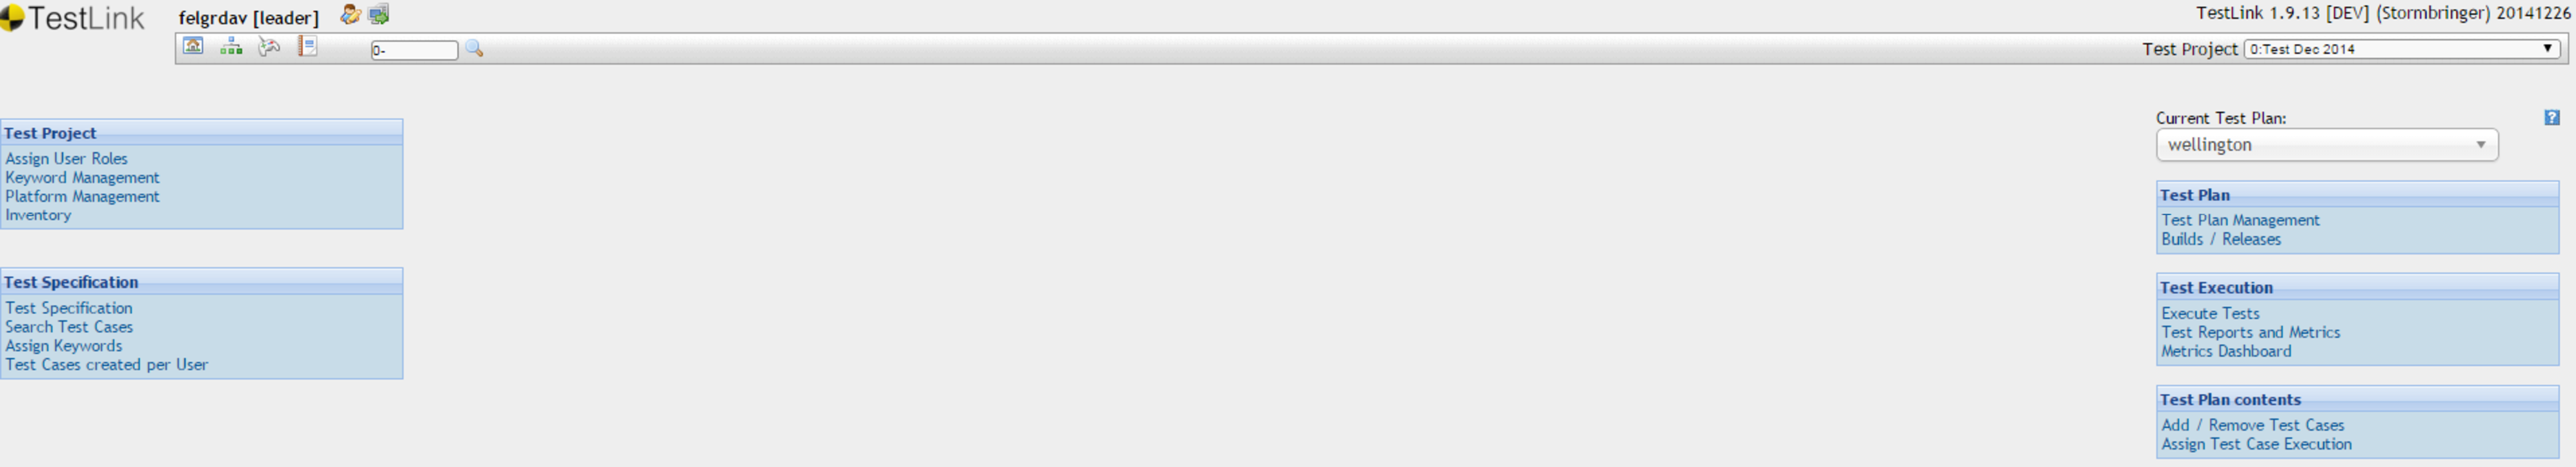
\includegraphics[width=\LW]{testlink_example}
  \caption{Příklad otevřené aplikace Testlink}
  \label{fig:testlink_example}
\end{figure}

Nástroj Testlink může být účinný v případě manuálního testování pro snadnou správu testů a reportování výsledků těchto testů. I v případě navrhovaném testovacím systému společnosti Conel by bylo možné systém nasadit. Jestliže by byl systém nasazen, byly by nutné úpravy tohoto systém k požadavkům automatického testování a speciálním požadavkům na modulárnost testovaných výrobků. Po krátkém zkoumání jsem zjistil, že úpravy pro automatické testování a úpravy k potřebám hierarchie  testovací laboratoře by byli rozsáhlé. Dále systém Testlink působí velmi nepřehledně. Díky těmto závěrům bylo rozhodnuto nepoužití nástroje Testlink pro spravování testů a reportování výsledků.

\section{Selenium}
Selenium je nástroj pro testování webových aplikací. Nástroj Selenium je také opensource projekt napsaný v jazyce Java. Selenium je dostupné ve čtyřech variantách a to Selenium IDE, Selenium RC, Selenium WebDriver a Selenium Grid. Selenium IDE je plugin do internetového prohlížeče Firefox. Dále Selenium RC, který si sám pouští internetové prohlížeče a provádí na nich testy. Testy je možné psát v jazycích Java, C, Python, Ruby, Perl, PHP a pro psaní těchto testů je připraveno přehledné API. Seleneium WebDriver usnadňuje psaní samotných testů na úkor nutnosti psaní všech testů na každý prohlížeč. Poslední Selenium Grid umožňuje paralélní spouštění testů na více strojích i počítačích.

\begin{figure}[h]
  \centering
  
\includegraphics[width=.1\LW]{selenium_logo}
  \caption{Logo produktu http://www.seleniumhq.org}
  \label{fig:selenium_logo}
\end{figure}

Selenium je dobrý nástroj pro testování webových aplikací. Nástroj bude určitě využitelný i pro testování webového rozhraní zařízeních testovaných v testovací laboratoři. V první fázi nasazení testovací laboratoře budou jednotlivé konfigurace měněni pomocí ssh a telnet přístupu do routeru. Jelikož tento nástroj více možností nepodporuje, tak nebude v první fázi nasazování testovacího zařízení využit.

\section{VectorCAST}
Nejlepším zkoumaným testovacím nástrojem byl komerční produkt VectorCAST od společnosti VECTOR Software. VectorCAST je platforma přímo určená k testování embedded zařízení podporující velkou škálu zařízení a testů.

\begin{figure}[h]
  \centering
  
\includegraphics[width=.4\LW]{vector_logo}
  \caption{Logo produktu http://www.vectorcast.com/}
  \label{fig:vector_logo}
\end{figure}

Samotný produkt je rozdělen do několika částí, které jsou dodávány zvlášť podle potřeb zákazníku a typu cílové testované aplikace. První dva programy se zabývají testováním jednotek a integračním testováním. První program je VevtorCAST/Ada, který je určen pro testování softwaru napsaném v jazyce Ada. Ada je robustní staticky typovaný programovací jazyk určený pro programování kritických aplikací. Tento jazyk v testovaných zařízeních nikdy nebyl použit a tak se dále tímto programem nebudu zabývat. Druhým programem určeným pro testování jednotek a integrační testování je VectorCAST/C++ určeným pro aplikace psané v jazycích C a C++.

VectorCAST/C++ je řešení pro automatizované testování jednotek a integrační testování. Tento nástroj přímo automatizuje vytváření unit testů pro samotný zdrojový kód. Nástroj je možné spustit nativně nebo na konkrétní cílové platformě. Pro spouštění na cílové platformě je potřeba nástroj VectorCAST/RSP, který bude popsán později. Další vlastností tohoto systému je jednoduché regresní testování softwaru, kdy je možné automaticky spouštět již vytvořené testy. Nástroj může pracovat ve dvou módech a to Source mód a Agile mód. První Source mód tvoří testy z modulů, které jsou již implementovány. Druhý Agile mód nepotřebuje pro tvorbu testů zdrojové kódy daného modulu, ale stačí mu pouze jeho hlavičkové soubory.

\begin{figure}[h]
  \centering
  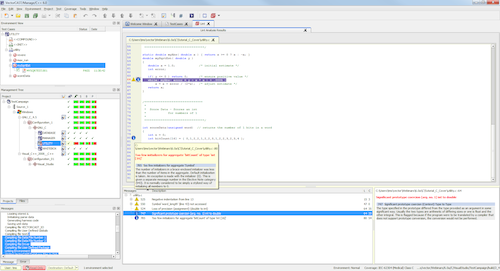
\includegraphics[width=\LW]{vector_example}
  \caption{Příklad otevřené aplikace VectorCast}
  \label{fig:vector_example}
\end{figure}

Pro lepší správu regresního testování slouží nástroj VectorCAST/Manage. Nástroj je vhodný pro vývoj aplikací s dlouhým životním cyklem, či s většími vývojovými týmy. Členové celého týmu mohou pohodlně spouštět regresní testy a sledovat jejich výsledky. Nástroj dále obsahuje podporu testování aplikace na více operačních systémech, více cílových platformách a různých konfiguracích. Testování stejného modelového případu ve všech možných situacích je důležité pro stoprocentní ověření systému. Nástroj umožňuje také funkci testování založené na změnách, kdy nástroj sleduje změny zdrojový kódů a spouští pouze testy modulů na kterých byli provedeny změny.

VectorCAST/Cover analyzuje využití kódu v průběhu systémového testování. Pomocí tohoto nástroje je možné zjistit, jaká část aplikace nebyla při samotném systémovém testování testována. Druhým nástrojem pro analýzu kódu VectorCAST/MCDC můžeme provést analýzu všech možných stavů a podstavů kam se aplikace psaná v jazyk C či C++ může dostat.

Testované aplikace je možné testovat přímo na cílové platformě pomocí již dříve zmíněného nástroj VectorCAST/RSP. V tomto nástroji je implementována široká škála kompilátorů. Pomocí VectorCAST/RSP lze stáhnout testovací postup přímo na cílovou platformu, kde jsou všechny testy prováděny a výsledky odeslány zpět testovacímu zařízení. Všechny kroky probíhají automaticky na pozadí bez interaktivity obsluhy.

Řešení pro testování embbeded aplikací VectorCAST a jeho všechny doplňující balíky jsou velmi silným nástrojem. Po detailní zkoumání tohoto nástroje a jeho funkcionalit nemohu ani tento nástroj doporučit pro účely automatické testování výrobků společnosti Conel. Hlavním důvodem nevhodnosti použití tohoto nástroje je potřeba zdrojového kódu k tvorbě jak testování jednotek, tak integračního testování. Firmware v testovaných výrobcích je z devadesáti procent tvořen opensource projekty. Tvorba takových testů na veškerém software by byla velmi dlouhá práce s nejasným výsledkem, taktéž projekt neobsahuje žádnou podporu systémového testování a návrh testů vzhledem k modulárnosti testovaných zařízení.

\section{Maveryx}
Maveryx je komerční řešení pro automatizované testování aplikací s grafickým uživatelským rozhraním. Tato aplikace podporuje testování aplikací napsaných v jazyce Java a aplikací pro operační systém Android. Aplikace Maveryx se nebude hodit k použití v testovacímu systému, ani pro řešení žádného mezikroku testování.

\section{Robot Framework}
Robot Framework je framework pro automatizované akceptační testování a vývoj řízený testy. Základní testovací možnosti lze rozšířit pomocí nových knihoven napsaných v jazyce Java nebo Python, pomocí kterých je možnost doplňovat nová klíčová slova.

\begin{figure}[h]
  \centering
  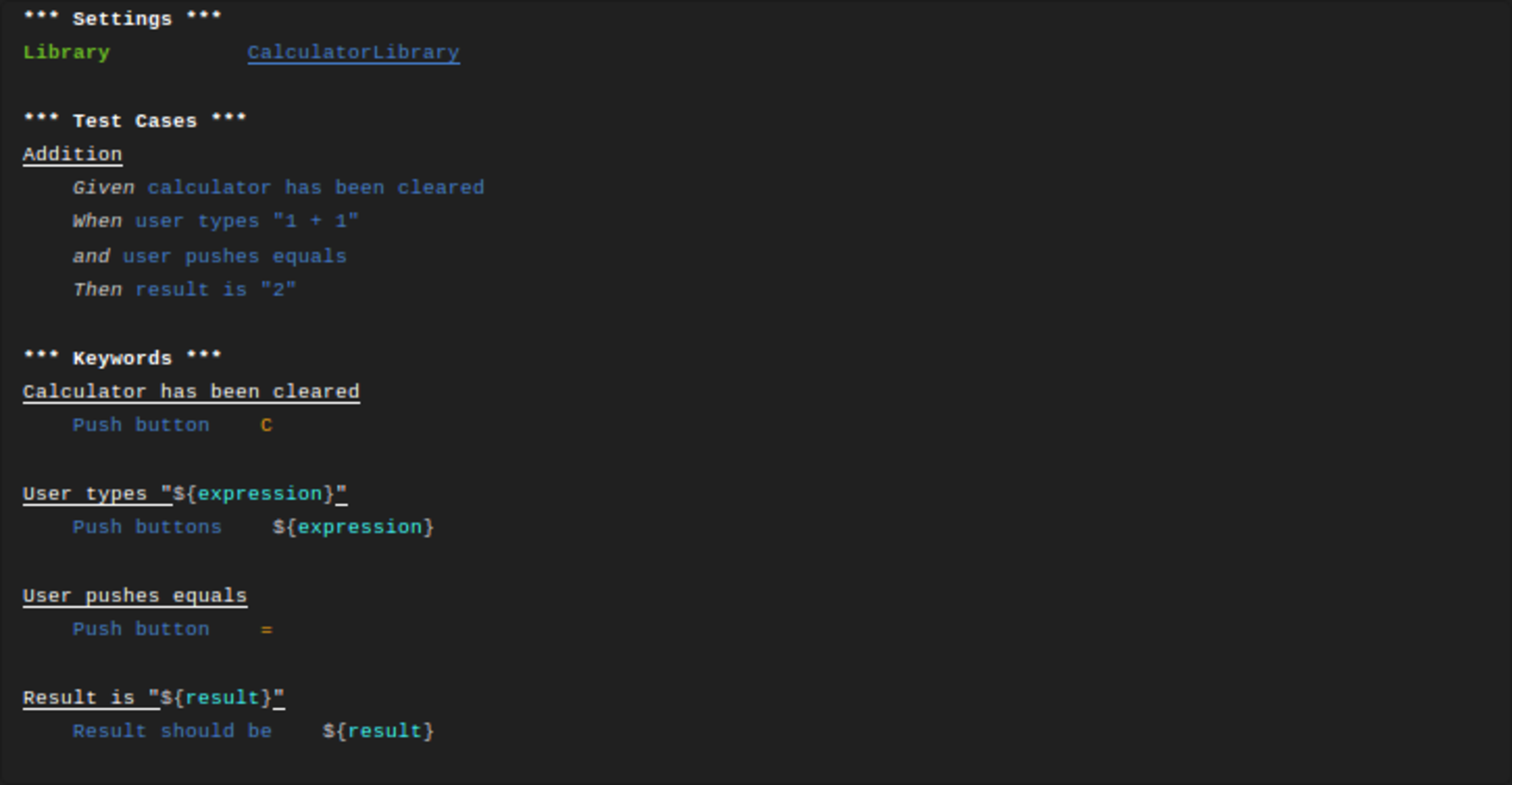
\includegraphics[width=\LW]{robot_example}
  \caption{Příklad testu ve framewotku http://robotframework.org/}
  \label{fig:robot_example}
\end{figure}

Robot Framework je pěkný příklad jak by mohl testovací framework vypadat. Specifické požadavky testovacího frameworku pro testování síťových embedded zařízení tento framework neobsahuje. Samozřejmě by se dali všechny knihovny dopsat pomocí přídavných knihoven a systém upravit k potřebám testovacího zařízení. Jednodušší cestou bude vzít dobré zkušenosti z testování tohoto frameworku a postavit vlastní API vhodné pro testování embedded aplikací.

Robot Framework je opensource projekt pod Apache Licencí 2.0. Robot Framework je nezávislý na operačním systému a aplikacích, jelikož jádro frameworku používá Python.

\section{Embedded Unit}
Embedded Unit je nástroj pro testování na úrovni testování jednotek. Nástroj je určen pro testování softwaru pro embedded aplikace. Jelikož tuto úroveň testování nebudu prozatím implementovat do testovacího systému, tak nebude tento nástroj prozatím využit.

\section{Linux Test Project}
Linux Test Project má za cíl testování stability, spolehlivosti a robustnosti Linuxového jádra a souvisejících funkcí. Tímto nástrojem bychom mohl testovat Linuxovou distribuci pro architekturu testovaných zařízení. S takto detailními testy se pro testovací laboratoř prozatím nepočítá, ale pro kvalitní testování výrobků se bude do budoucna hodit.

\section{Ostatní aplikace}
API pro vytváření jednotlivých testů bude využívat různé, převážně opensource programy ze světa síťových technologií. Například Curl pro komunikaci mnoha síťovými protokoly Všechny tyto použité programy budou popsány v kapitole věnující se API testovacího systému.

\endinput

  \chapter{Návrh testovací laboratoře}

Pro testování všech výrobků společnosti Conel nejdříve navrhnu strukturu testovací laboratoře.  Testovací laboratoř bude síť obsahující všechny výrobky společnosti Conel, různá příslušenství připojené k jednotlivým výrobkům, testovací server a konfigurovatelné switche.

\section{Testovací server}
Jádrem testovací laboratoře bude server na kterém poběží všechny testovací aplikace. Testovaci server bude výkonější počítač s parametry procesor Intel core i7, 16GB RAM a 512GB SSD disk. Pro účely testování bude server osazen dvěma ethernetovými rozhranímy pro komunikaci s testovanými výrobky a jedním ethernetovým rozhraním pro konektivitu serveru do firemní sítě. Server dále má osazeno jedno WiFi rozhraní pro testování WiFi výrobků.  Operační systém tohoto serveru jsem zvolil Ubuntu server, jelikož operační systém Ubuntu je používán k vývoji většiny výrobků.

\section{Konfigurovatelné switche}
Pro propojení všech výrobků s testovacím serverem budou použity dva konfigurovatelné 48 portové switche od firmy CISCO. Dva switche byly zvoleny kvůli velké ceně switchů nad 48 portů. Konfigurovatelné switch budou potřeba pro změnu síťové infrastruktury v průběhu testu. Každý switch bude připojen k jednomu ethernetovému rozhraní serveru, dále budou switche navzájem propojeny. Nejen všechny výrobky, ale každé fyzické ethernetové rozhraní bude připojeno do switche a pomocí VLAN bude vytvořena požadovaná testovací síť.

\section{Výrobky společnosti Conel}
Zařízení které tvoří přes devadesát procent prodeje firmy Conel jsou bezdrátové routery a i tato zařízení budou testovány v testovací laboratoři. Bezdrátové routery tvoří celkem čtyři modelové řady, které dále obsahují jednotlivé výrobky podle technologie bezdrátového připojení a počtu rozhraní.

\subsection{Řada routerů v0}
Takzvaná nultá řada routerů obsahuje pouze dvá výrobky. Prvním ER75i disponující EDGE technologií, jedním ethernet rozhraním možností a osazením jednoho volitelného portu.  Druhým výrobkem této řady je UR5, který se liší pouze bezdrátovou technologií. Místo EDGE technologie disponuje rychlejší UMTS technologií. Oba tyto výrobky jsou postaveny na uClinuxu a i přes jejich stáří se firmware stále udržuje.

\subsection{Řada routerů v1}


\subsection{Řada routerů v2}
\subsection{Řada routerů v3}

\section{Volitelné porty}
\subsection{Port LAN}
\subsection{Port WiFi}
\subsection{Port RS232}
\subsection{Port RS485/422}
\subsection{Port CNT}

\section{Cisco router}




\endinput
  
  \chapter{Testovací program}
Testovací systém běžící na serveru testovací laboratoře se skládá z několika samostaných částí. Základem celého systému je databáze uchovávající všechna informace struktuře testovací laboratoře data s výsledky jednotlivých testů. Program testlab se stará o celý průběh testování. Několika málo přepínači lze nastavit průběh testování. Další součástí je sada programů nazývající se testovací API. Tyto programu usnadňují psaní jednotlivých testů. Nedílnou součástí testovacího systému jsou testovací skripty, které lze rozdělit na skripty pro stáhnutí projektu, kompilaci projektu, testování výrobku a úklid projektu. Poslední součástí testovacího systému je webový interface pro sledování výsledků testování a nastavování chování testovacího systému.

\section{Adresářová struktura testovacího systému}

Jednotlivé částí testovacího systému jsou rozloženy v adresářové struktuře serveru následovně. Testovací program a testovací API jsou umístěny v adresáři /usr/bin. Sdílené knihovny pro testovací program a jednotlivé programy testovacího API jsou umístěny v a

\begin{figure}[h]
  \centering
  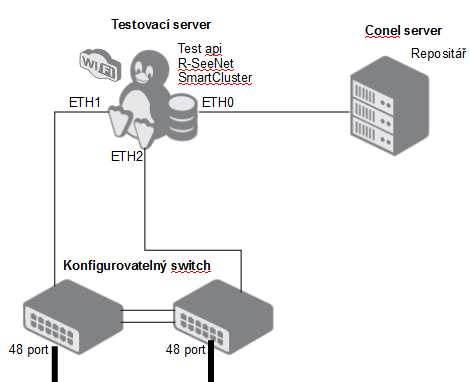
\includegraphics[width=.4\LW]{server_switch}
  \caption{Adresářová struktura testovacího systému}
  \label{fig:server_switch}
\end{figure}

\section{Struktura databáze}

\section{Popis programu}

O průběh celého testu se stará program testlab. Testlab je program psaný v jazyc C. Program po spuštění otevře systémový log pro možnost logování chyb do systémového logu. Filtrováný systémový log by měl později být zobrazován na webowém rozhraní testovacího systému. První hláškou do systémového logu je informace o spuštění programu testlab, daným uživatelem a v určený čas. Po otevření systémového logu program rozebírá parametry na příkazové řádce. Parametry jsou rozebíráný pomocí funkce getopts. Pomocí parametrů lze ovlivnit chování programu testlab !!!!!DOPLNIT PARAMETRY!!!!!!

\begin{figure}[h]
  \centering
  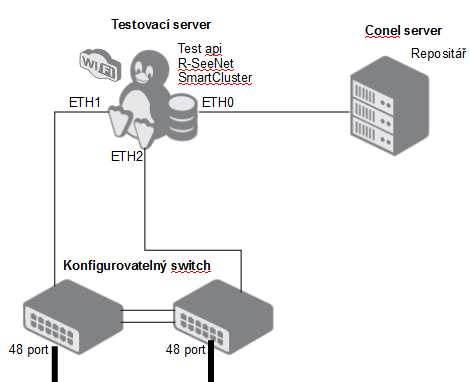
\includegraphics[width=.4\LW]{server_switch}
  \caption{Zapojení testovacího serveru a switchů}
  \label{fig:server_switch}
\end{figure}


Nyní se provádějí přípravné kroky pro samotné testování. Nejdříve je vytvořen nový release firmwaru a následně vložen do databáze. V projektovém adresáři je vytvořen nový adresář se stejným názvem jako identifikační číslo testovaného releasu.

\section{Checkout}
\section{Compile}
\section{Test router}
\section{Test tunel}
\section{Clean}
\section{Remote server}
\subsection{Telnet}
\subsection{SSH}

\endinput

  \chapter{Uživatelský interface}


\endinput

  \chapter{API pro psaná testů}


\endinput

  \chapter{Návrh testů pro Conel routery}


\endinput

  \chapter{Testovací laboratoř v praxi}


\endinput

  \chapter{Návrhy na budoucí rozšíření}


\endinput

  \chapter{Závěr}


\endinput



  %\startAppendices
  %  \chapter{Appendix}
Some introductory text\dots

\section{Section}
Another text\dots

\endinput
%%
%% End of file `app01.tex'.

  %\stopAppendices
\stopBodyMatter

\startBackMatter
  \PrintBibliography
  %\PrintIndex % define index entry in the text by: \index{word}
\stopBackMatter

\end{document}

\endinput
